

% \begin{frame}[c]{}
%     \centering
%     \begin{figure}
%         \centering
%         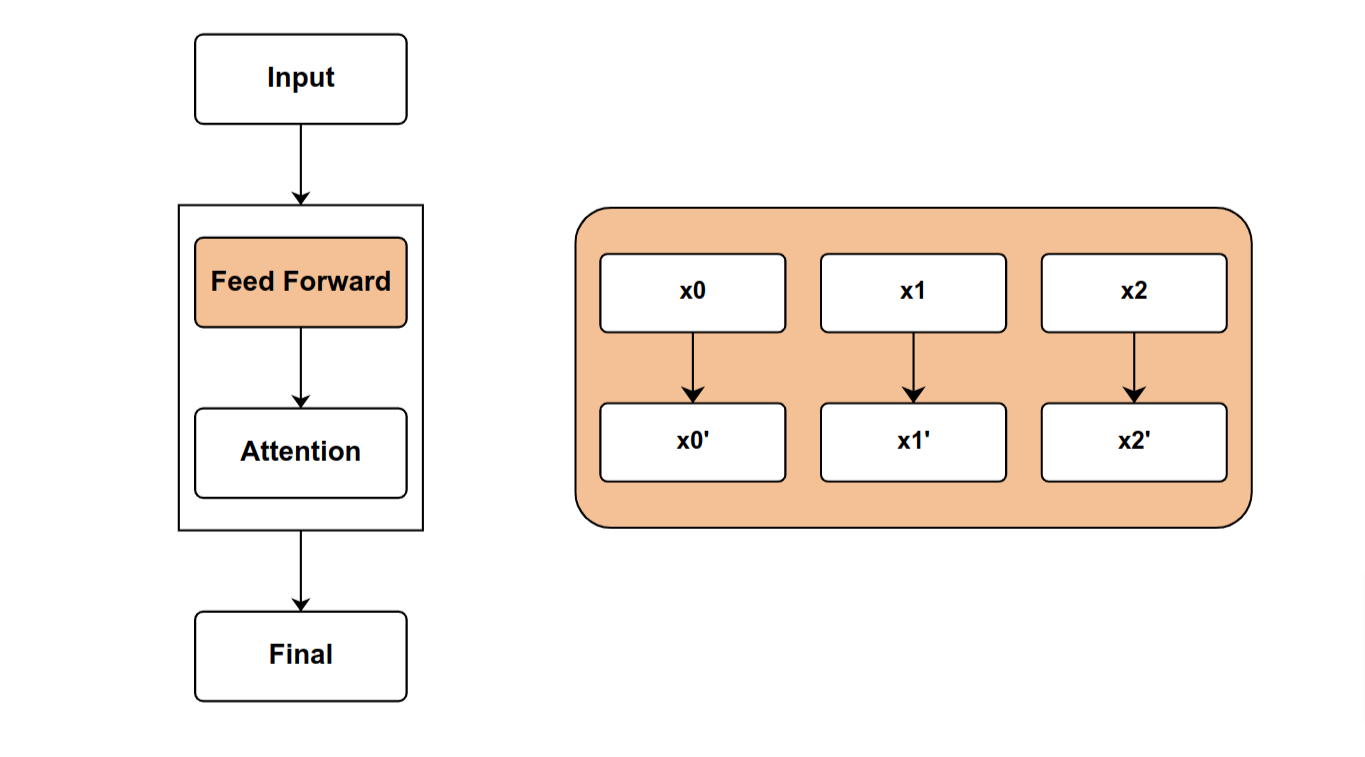
\includegraphics[height=0.9\textheight]{Figs/FeedForward.png}
%         \label{fig:my_label}
%     \end{figure}
% \end{frame}

\begin{frame}[c]{Transformers for Sequence Modeling}
    \centering
    \begin{columns}
    \begin{column}{0.3\textwidth}
        Repeated components 
        \vspace{0.5cm}
        
            \begin{itemize}
                \item Feed Forward

                \item Attention 
            \end{itemize}
    \end{column}        
    \begin{column}{0.7\textwidth}

    \begin{figure}
        \centering
        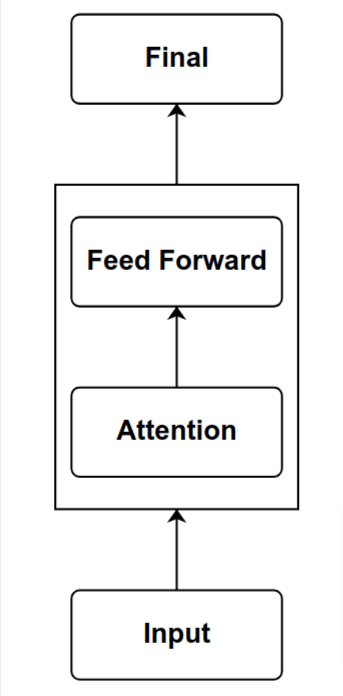
\includegraphics[height=0.8\textheight,  clip,trim={0.1cm 0.1cm 0.1cm 0.1cm}]{Figs/out.png}
        %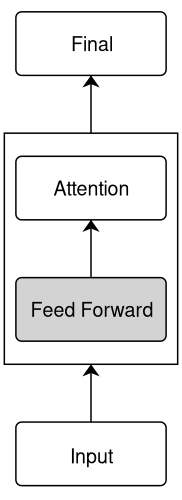
\includegraphics[height=0.8\textheight]{Figs/out2 (1).png} \label{fig:my_label}
    \end{figure}
    \end{column}
    \end{columns}        

\end{frame}

\begin{frame}{Feed Forward}
    \begin{itemize}
        \item Acts on each position independently. 
    \end{itemize}
    \begin{figure}
        \centering
        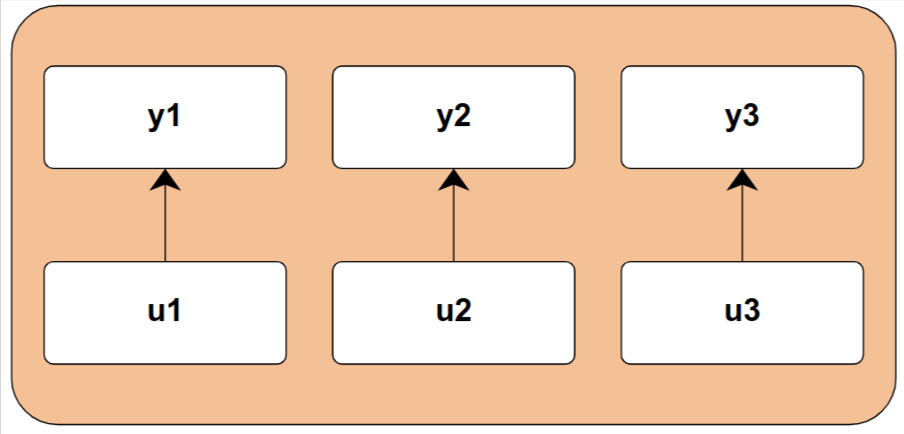
\includegraphics[height=0.5\textheight, clip,trim={0.1cm 0.1cm 0.1cm 0.1cm}]{Figs/out4.png}
    \end{figure}
\end{frame}

\begin{frame}[c]{Attention} 
    \begin{itemize}
        \item Fully connected interactions.
    \end{itemize}

    \centering
    \begin{figure}
        \centering
        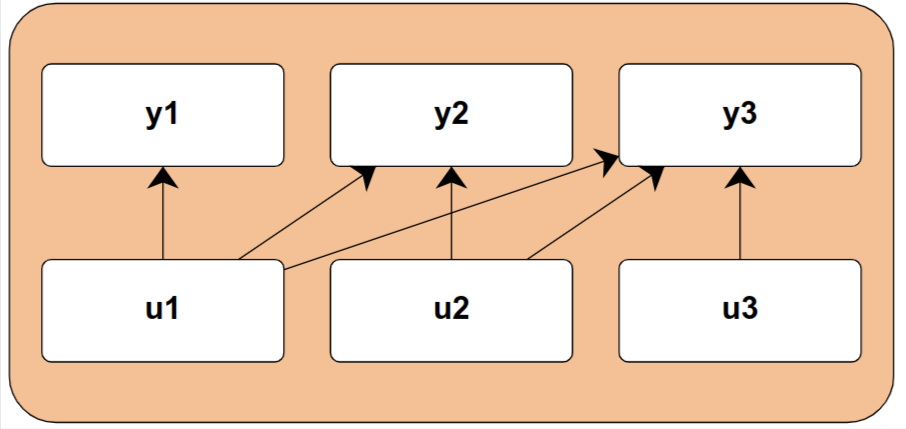
\includegraphics[height=0.5\textheight,  clip,trim={0.1cm 0.1cm 0.1cm 0.1cm}]{Figs/out5.png}
        \label{fig:my_label}
    \end{figure}    
\end{frame}


% \begin{frame}{Attention Matrix}
%         \centering
%     \begin{itemize}
%         \item Schematic of interactions at each layer (quadratic)
%     \end{itemize}

    
%     \begin{figure}
%         \centering
%         % 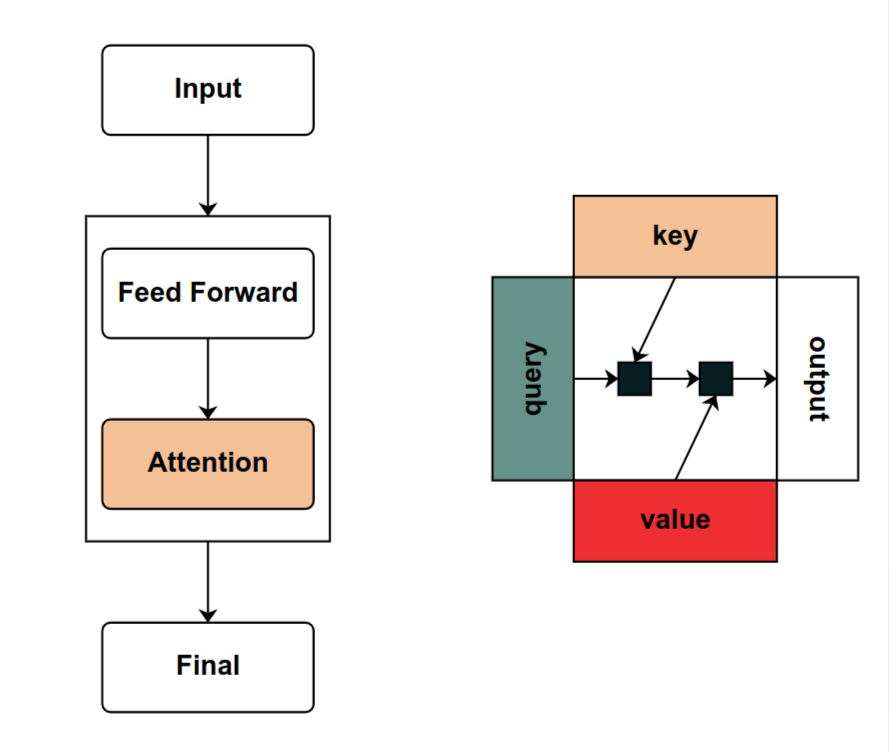
\includegraphics[height=0.7\textheight,clip,trim={14cm 3cm 0.5cm 3cm}]{Figs/Attention.png} \hspace{1cm} 
%         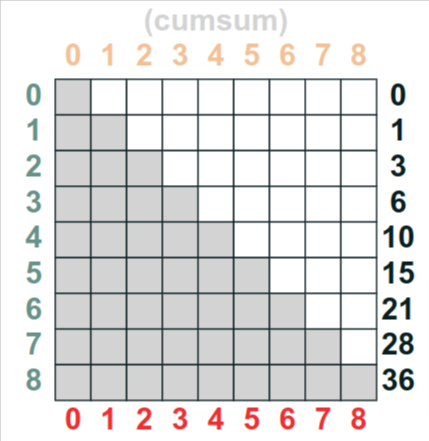
\includegraphics[height=0.7\textheight, clip, trim={1.5cm 1.3cm 0.1cm 0.1cm}]{Figs/Cumsum.png}
%         \label{fig:my_label}
%     \end{figure}
% \end{frame}


\begin{frame}[c]{Task: Language Generation}
    \centering
    Predict the next word.
    \vspace{1.5cm}
    

    \structure{Final:}  The dog walked to the \textcolor{red}{park}
    
    \vspace{1.5cm}
    
        \textcolor{blue}{Input:} The dog walked to the  \textcolor{red}{?}

\end{frame}

\begin{frame}[c]{Task: Long Range Arena (ListOps)}
    \centering
    Calculate the equation ($\uparrow$=max $\downarrow$=min)
    \vspace{1.5cm}

    
    \structure{Final:} [ $\uparrow$ 2 9 [ $\downarrow$ 4 7 ] 0 ] \textcolor{red}{9}
    
    \vspace{1.5cm}

    
    \textcolor{blue}{Input:}  [ $\uparrow$ 2 9 [ $\downarrow$ 4 7 ] 0 ] \textcolor{red}{?}
\end{frame}



\begin{frame}[c]{Attention Matrix}

    \centering

    \begin{center}
        All quadratic interactions possible.
    \end{center}
    
    \begin{figure}
        \centering
        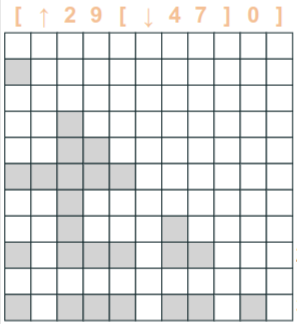
\includegraphics[height=0.6\textheight, clip,trim={0.1cm 0.1cm 0.1cm 0.1cm}]{Figs/Complex.png}
       \label{fig:my_label}
    \end{figure}
\end{frame}

\begin{frame}[c]{Attention for Realistic Examples}
    \centering
     \begin{center}
    Listops goes to 2,000 steps. This is 100.
    \end{center}

    \begin{figure}
        \centering
        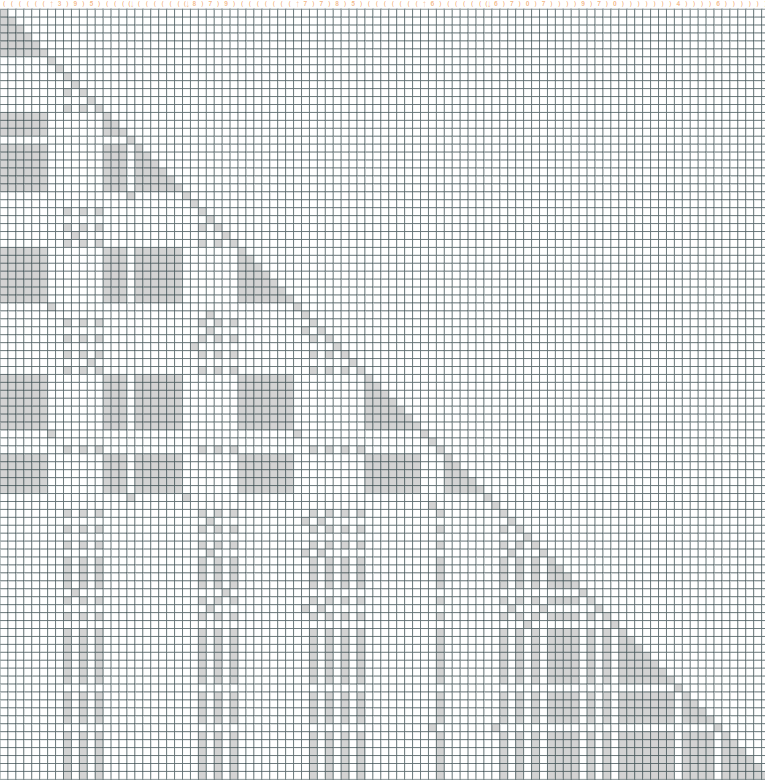
\includegraphics[height=0.6\textheight, clip,trim={0.1cm 0.1cm 0.1cm 0.1cm}]{Figs/big.png}
       \label{fig:my_label}
    \end{figure}
\end{frame}




    